% !TEX root = main.tex
\section{交易验证}
\label{sec:tx_verification}
\subsection{基础}
基于第\ref{sec:leader_election}章,在已选举出提案者的情况下,交易验证对提案者的出块进行验证,该问题可以抽象为分布式系统中的状态机复制问题\cite{pass2017rethinking}。

%首先给出拜占庭环境下交易验证的相关定义和特性。


%对于节点集合$V$\footnote{类似于定义\ref{def:leader_election},此处$V$可为有限或无限集合。},
首先我们给出拜占庭容错的状态机复制问题定义。
\begin{definition}
(拜占庭容错状态机复制)对于接受节点集合$A$,其中最多有$f$个拜占庭节点(即最少有$n_a-f$个诚实节点),所有接受节点必须从提案中最终做出决策,并且满足下述条件:
\begin{itemize}
	\item 一致性(Agreement):所有诚实节点的决策必定相同。
	\item 可终止性(Termination):所有诚实节点在有限的时间内结束决策过程。
	\item 有效性(Validity)\footnote{部分研究中将可终止性和有效性描述为活性(Liveness)。}:选择出的决策值必须来自某个有效的提案。
\end{itemize}
\end{definition}

根据FLP定律,在完全异步网络拜占庭环境下,不存在确定性的算法满足上述条件\cite{fischer1982impossibility}。因此现有区块链交易验证算法都是同步(或者所谓的半同步)网络拜占庭环境下的状态机复制算法\cite{gilad2017algorand,castro1999practical}。

\subsection{性质分析}
对于共识机制,除了上述必须满足的特性之外,我们讨论另一个重要性质,最终性(Finality)。在区块链共识系统中,最终性是指由诚实接受节点决策通过的区块状态不会被改变,最终性又被称为绝对最终性(Absolute Finality),对应地,存在一定概率使已通过区块状态改变称之为概率最终性(Probabilistic Finality)\footnote{Finality in Blockchain Consensus, https://medium.com/mechanism-labs/finality-in-blockchain-consensus-d1f83c120a9a}。

交易确认机制根据块是否具有最终性划分为链式协议和基于投票协议\cite{wang2019survey}。

\subsubsection{链式协议}
链式交易验证则仅满足概率最终性,即随着链结构的增长交易状态改变的概率逐渐降低,但永远无法达到零,即仍然存在被改变可能。


\subsubsection{投票协议}
投票式交易验证满足最终性,即交易一旦完成验证则不可能发生改变。对应地,需要指出的是,即便是基于投票的验证协议,其底层数据结构仍可以采用链式区块结构。

从安全性角度,我们不希望已经验证的交易会存在修改的可能,即出现双重支付(Double-Spending)或者长距离攻击(Long-Range Attack)。虽然比特币等采用链式验证协议的系统认为随着最长链的增长其被扭转概率会非常低,但实际上目前比特币网络中排名前四的矿池已经占据了全网$50\%$以上算力\footnote{https://www.blockchain.com/pools.},这意味着其安全性是由矿池决定而并非系统本身。因此理论上安全的区块链系统必须满足最终性。

同时,随着数据的不断增长,一些普通节点可能无法负担庞大的数据量,因此最终性可以减少数据的存储。最后,考虑到未来的分片设计,数据分片需要最终性作为基础。

综上,我们采用基于投票机制的设计,保证交易验证的最终性。


\subsection{已有投票策略分析}
首先我们对目前基于投票的验证策略进行简单分析。根据是否需要验证节点进行身份验证,我们将投票策略分为授权投票和无授权投票,通常来说分别适用于联盟链和公链。

\subsubsection{授权投票策略:PBFT}
PBFT协议\cite{castro1999practical}最早并不是用于区块链,协议中负责提案的节点称之为主节点(Primary),即领袖节点。在已经指定领袖节点的情况下,提案验证过程包括下面3步:
\begin{itemize}
	\item PRE-PREPARE:主节点在收到请求后向所有副本节点广播与准备消息,其格式为$\langle \langle PRE-PREPARE,v,n,d \rangle_{\sigma p},m \rangle$,其中$v$是视图编号,$n$是消息序号,$d$是消息摘要,$m$为请求消息,$\sigma p$为主节点$p$的签名;
	\item PREPARE:一旦副本节点$i$接受预准备消息则进入准备阶段,同时该节点向所有副本节点发送准备消息$\langle PREPARE,v,n,d,i\rangle_{\sigma i}$。当节点$i$收到$2f$个从不同副本节点发来与$PRE-PREPARE$相匹配的$PREPARE$消息,则定义$prepared(m,v,n,i)$为真;
	\item COMMIT:当$prepared(m,v,n,i)$为真时,副本节点$i$将$\langle COMMIT,v,n,D(m),i\rangle$广播至其他副本节点,进入确认阶段。对节点$i$而言,$prepared(m,v,n,i)$为真且$i$已经接受了$2f+1$个$COMMIT$消息与$PRE-PREPARE$消息一致则定义$committed-local(m,v,n,i)$为真。而存在$f+1$个正常副本节点集合使得其中所有副本节点$i$的$prepared(m,v,n,i)$为真,则定义$committed(m,v,n)$为真。
\end{itemize}

\textcolor{gray}{预准备阶段和准备阶段确保所有正常节点对同一个视图中的请求序号达成一致。而确认阶段保证了所有正常阶段对本地确认的请求序号达成一致,及时这些请求在每个节点的确认处于不同的视图。}

不难发现,在PBFT策略中,验证节点为固定的集合,并且所有节点身份公开,在其发布PREPARE消息后其决策也公开可见,因而在其发布正常COMMIT消息前存在被攻击或者贿赂可能。所以对于采用PBFT算法的系统,无法适用于无授权环境。

\subsubsection{无授权投票:Algorand}
%无授权场景下节点会动态加入离开,同时由于节点没有身份认证,

不同于PBFT,Algorand\cite{gilad2017algorand}属于无授权场景共识 协议,对应地,Algorand在领袖选举和交易验证中均采用了基于VRF的随机抽取策略。这里重点分析其交易验证部分。

Algorand验证的核心算法$BA\bigstar$来自于\cite{miller2016honey},具体如下:
\begin{itemize}
	\item Reduction:该步骤的目标是将需要达成共识的多个区块转化为对某一特定区块或者空块二选一达成共识;
	\item BinaryBA$\bigstar$:基于Reduction的输出,在特定区块和空块之间达成共识。在$Maxstep$轮中没有达成共识则认为网络状况出现问题。
\end{itemize}

需要注意的是,在Reduction和BinaryBA$\bigstar$中,都需要多次执行$CommitteeVote()$和$CountVotes()$操作,即投票和计票。这里重点分析前者,$CommitteeVote()$输入包括$(ctx,round,step,\tau,value)$,其中$ctx$为环境变量(包括当前账本信息以及当前种子等等),$round$表示当前轮数,$step$表示执行当前计票操作的步骤(例如Reduction-1),$\tau$表示抽签比例参数,$value$表示投票区块。

验证节点执行$CommitteeVote()$时需要先执行$Sortition()$即通过抽签判断自己是否有资格参与投票,不难发现,在给定$round$和随机种子($ctx.seed$)情况下,每个验证节点每次执行$Sortition()$的结果固定。因此实际上在Reduction和BinaryBA$\bigstar$过程中,仍然是同一批节点在参与投票,并且在Reduction中的第一次$CommitteeVote()$之后,所有投票的节点身份已经曝光,因此也存在被攻击或者贿赂的风险。

Algorand假设在整个$BA\bigstar$过程中所有验证节点不会改变投票选择,在保证三分之二诚实节点的情况下,如果收不到足够的投票则问题一定出在网络上\footnote{Algorand假设网络最终会收敛于同步模型}。但由于诚实节点仍可能会被攻击或者贿赂,我们认为该算法仍然存在问题。


\subsection{投票模型}
目前关于电子投票(Electronic Voting)的研究中\cite{kiayias2002self},除去传统的隐私性(Privacy)、公平性(Fairness)和健壮性(Robustness)需求,理想的电子投票还需要满足如下要求:
\begin{itemize}
	%\item 隐私性:
	%\item 健壮性:
	%\item 公平性:
	\item 可校验性(Universal-Verifiability):任何第三方都可以验证最后的投票结果是否正确统计了合法选票\footnote{另有原子可校验性描述仅投票者可以验证投票结果是否正确统计了合法选票。};
	\item 无收据性(Receipt-Freeness):投票者无法向第三方证明其所投的选票内容;
	\item 无争议性(Dispute-Freeness):任何第三方都可以验证协议的参与方是否正确执行了协议;
	\item 自计票性(Self-Tallying):任何第三方可以进行计票,而不需要可信第三方或者投票者的参与;
	\item 完善保密性(Perfect Ballot Secrecy):假设存在$n$个选民,任何$t$个($t<n$)投票者的投票结果只有剩余$n-t$个投票者串通起来才能知道。
\end{itemize}

而对于共识机制中的投票系统,由于不存在可信的第三方机构,每个验证节点既是投票者也是计票者\textcolor{red}{(即所谓的"all voters are talliers")},因此其必须满足可校验性和自计票性。\textcolor{red}{论文\cite{kiayias2002self}指出在大规模的投票系统中,并不需要满足完善保密性。}

现有大多数基于投票的共识机制都无法满足无收据性和无争议性,具体地来说,对于拜占庭验证节点,虽然无法伪造或篡改其他人的消息\footnote{通常而言,我们认为现有的签名算法可以保证信息无法篡改或者伪造。},但仍可能出现如下恶意行为:

\begin{itemize}
	\item 恶意投票:恶意验证者不发布任何投票或者对其他验证者发布不同的投票,例如对部分验证者发布$\langle pk_i,sign_{sk_i}(t,h(B_1),\pi_i) \rangle$,而对另一部分验证者发布$\langle pk_i,sign_{sk_i}(t,h(B_2),\pi_i) \rangle$,$B_1 \neq B_2$。
	\item 割裂网络:在采用Gossip协议传输的网络中,恶意节点可能在收到其他节点的投票后不向其他节点转发该信息,导致原有投票信息无法广播到所有节点。
	\item 共谋:恶意节点在投票前或者投票过程中得知其他验证者身份,从而贿赂其他验证者使其投票决策发生变化。
\end{itemize}

\textcolor{red}{作为分布式系统,区块链中所有验证节点通过P2P方式进行通信,因此任何节点在投票过程中都无法检验其他节点是否正确执行协议,即在投票过程中无争议性无法保证。}\footnote{尽管Casper通过Slash机制实现了检点的互相监督,但恶意行为被发现是基于交易已经上链的前提。}在这种情况下,恶意投票和割裂网络将变得可行。这两种行为会导致决策无法收敛,从而影响共识的活性。%目前的投票共识往往通过监督检举的方式来减少恶意投票和割裂网络行为\cite{buterin2017casper}。

共谋行为则违背了无收据性,\textcolor{red}{现有大部分投票共识都没有考虑拜占庭节点的共谋行为}并且假设系统中拜占庭节点比例低于某个阈值(例如三分之一),而实际上,由于共谋行为的存在,系统中拜占庭节点比例会更高。

%即便,其仍可能通过共谋导致潜在的安全问题。
我们认为理想的投票机制应该抵抗上述三种恶意行为。首先,我们给出投票流程中的相关定义:

\begin{definition}
	(注册)对于任何期望参与验证过程的节点$i$,执行操作$R(s_i,\varepsilon)$,$s_i$为节点$i$的状态,$\varepsilon$为额外证明输入\textcolor{gray}{(通常为某个随机数)},$R$输出为
\end{definition}

\begin{definition}
(投票) 对于验证节点$i$,在接受某提案区块$B$后,满足$V(B,t)=1$的情况下,对所有验证节点广播消息$\langle pk_i,sign_{sk_i}(h(B),\pi_i) \rangle$。其中$sign_{sk_i}(\cdot)$表示基于节点$i$私钥的签名,$h(B)$表示提案区块$B$的哈希值,$\pi_i$表示验证节点$i$的投票效益证明。
\end{definition}

\begin{definition}
	(验票)
\end{definition}

\begin{definition}
(计票) 对于验证节点$j$,对所有验证节点广播消息$\langle pk_i,sign_{sk_i}(h(B),\pi_i) \rangle$。其中$sign_{sk_i}(\cdot)$表示基于节点$i$私钥的签名,$h(B)$表示提案区块$B$的哈希值,$\pi_i$表示验证节点$i$的投票效益证明。
\end{definition}


\subsection{补充:投票效益}
除了投票过程中可能出现的攻击,对于投票效益的计算,我们认为也可能存在如下潜在的安全问题:

\begin{itemize}
	\item 女巫攻击:投票过程必须能够抵抗女巫攻击(Sybil Attack),解决方法可以是通过设置准入门槛或者将投票效益与参与者的资产挂钩。
	\item Nothing-at-Stake:通常而言区块链共识的投票是根据参与者的持有(或抵押)的资产计算所得,在没有投票成本的情况下,验证者更倾向分散其投票效益。一种解决方法是引入投票成本,或者对于分散投票行为作出惩罚\cite{buterin2017casper}。	
	%\item 共谋:为防止贿选以及共谋现象(Colluding),投票前投票节点身份不应曝光,同时在每次投票后(例如公布对某个区块的签名公证),其将丧失投票资格,直至再次入选委员会。
	%\item 延迟:尽管任何共识机制都需要保证在有限时间内结束决策,但我们仍希望投票能够快速达成一致,从而减少交易的确认延时(confirmation delay)。
\end{itemize}


\begin{figure}
\centering
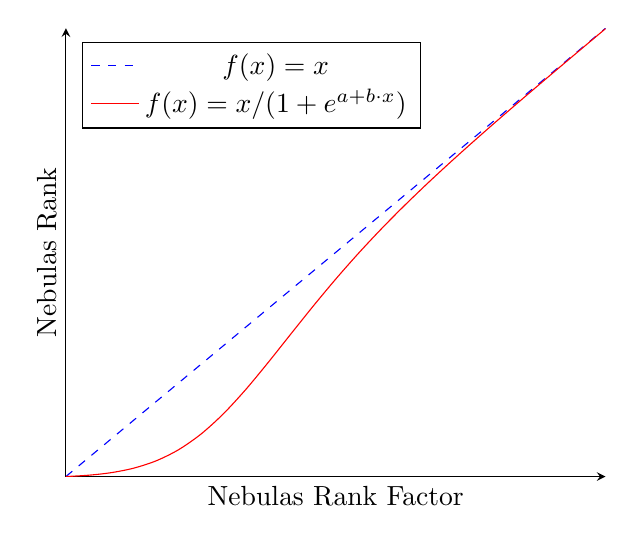
\begin{tikzpicture}[
    declare function={func(\x,\mu) = (\x / (1 + exp(\mu-\x)));},
    declare function={linefunc(\x) = \x;}
]
\begin{axis}[
    axis lines=left,
    enlargelimits=upper,
ticks=none,axis x line=bottom,axis y line=left,xlabel={Nebulas Rank Factor},
  ylabel={Nebulas Rank},
      legend pos=north west,
legend style={fill=none}
]
\addplot [dashed, domain=0:10, blue] {linefunc(x)};
\addplot [smooth, domain=0:10, red] {func(x,3)};
\addlegendentry{$f(x)=x$}
\addlegendentry{$f(x)=x/(1 + e^{a + b\cdot x})$}
\end{axis}
\end{tikzpicture}
\caption{The curve of the Nebulas Rank function \label{fig-nr}}
\end{figure}